% file: consistency-model/pram-3proc.tex

\documentclass[tikz]{standalone}

\usetikzlibrary{positioning, shapes, calc, backgrounds, fit}

\newcommand{\po}[2]{\draw [->, thick, violet] (#1) to node[above] {so} node[below, teal] {vis} (#2);}
\newcommand{\rw}[2]{\draw [->, thick, teal] (#1) to node[below, sloped] {vis} (#2);}

\begin{document}
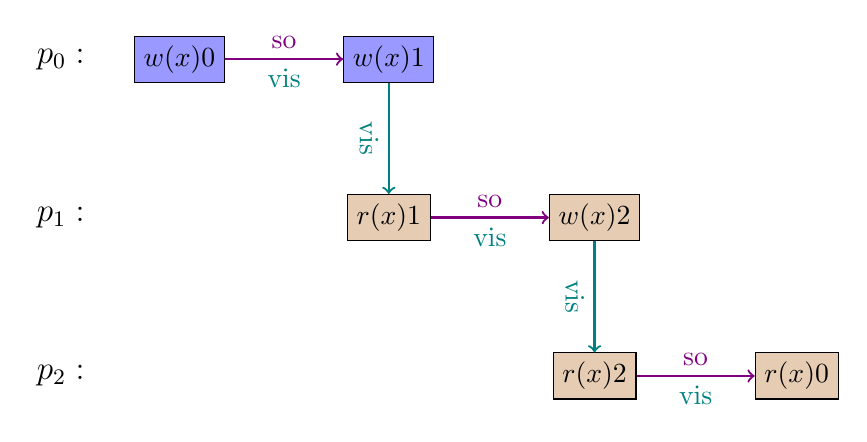
\begin{tikzpicture}[
    wop/.style = {rectangle, fill = blue!40, draw}, 
    rop/.style = {rectangle, fill = brown!40, draw}, 
    process/.style = {font = \large}, 
    rw/.style = {->, thick, teal}]

  \node (p0) [process] {$p_0:$}; 
  \node (wx0) [wop, right = 0.5cm of p0] {$w(x)0$};
  \node (wx1) [wop, right = 1.5cm of wx0] {$w(x)1$};
  \po{wx0}{wx1}

  \node (p1) [process, below = 1.5cm of p0] {$p_1:$}; 
  \node (rx1) [rop, at = (p1 -| wx1)] {$r(x)1$};
  \node (wx2) [rop, right = 1.5cm of rx1] {$w(x)2$};
  \po{rx1}{wx2}

  \node (p2) [process, below = 1.5cm of p1] {$p_2:$}; 
  \node (rx2) [rop, at = (p2 -| wx2)] {$r(x)2$};
  \node (rx0) [rop, right = 1.5cm of rx2] {$r(x)0$};
  \po{rx2}{rx0}

  \rw{wx1}{rx1}
  \rw{wx2}{rx2}
\end{tikzpicture}
\end{document}
